\documentclass[conference]{IEEEtran}

\usepackage{cite}
\usepackage{amsmath,amssymb,amsfonts}
\usepackage{graphicx}
\usepackage{textcomp}
\usepackage{xcolor}
\usepackage{booktabs}
\usepackage{multirow}
\usepackage[hidelinks]{hyperref}
\usepackage{subcaption}
\usepackage{siunitx}

\sisetup{detect-weight=true, detect-family=true}

% TODO marker so any unfilled number is obvious in the build
\newcommand{\todo}[1]{\textcolor{red}{\textbf{[TODO: #1]}}}
\newcommand{\tbd}{\textcolor{red}{\textbf{tbd}}}

\begin{document}

\title{Deep Learning for Vessel Segmentation in Cerebral CTA:\\Topology-Aware and Reconstruction-Aware Loss Functions}

\author{
\IEEEauthorblockN{Samih Tharwat Amer}
\IEEEauthorblockA{Whiting School of Engineering\\
Johns Hopkins University\\
}
}

\maketitle

% ============================================================================
\begin{abstract}
Accurate segmentation of cerebral vasculature from computed tomography angiography (CTA) is essential for surgical planning of stroke and intracranial aneurysms, yet standard Dice + cross-entropy objectives produce topological failures---severed vessels that render segmentations clinically unusable despite high aggregate scores. We present a controlled seven-way loss ablation: a 3D U-Net is trained from scratch on TopCoW 2024 (125 CTA volumes, 13 Circle of Willis classes) under a topology-aware family (Dice+CE, +clDice, +Skeleton Recall), a reconstruction-aware family (+SSIM, +MSE-on-distance-transform, +VGG perceptual), and a clDice+SSIM combination. All configurations share identical architecture, hyperparameters, and hardware (8$\times$A100 GPUs); only the loss varies. We additionally introduce three reconstruction-style metrics (3D-SSIM, PSNR, Fr\'{e}chet Feature Distance) to evaluate each model on an axis orthogonal to overlap and topology. Paired Wilcoxon tests across the 25 validation cases (Holm-Bonferroni corrected) reveal a sharper picture than the means alone: clDice is significantly better than five of six other configurations on the centerline-Dice metric (excluding Combo) and produces the lowest Betti-0 numerically, but on DSC only clDice vs.\ Skeleton survives correction (capturing Skeleton's fragmentation cost), and binary-mask reconstruction metrics cluster within noise. Note: our SSIM/PSNR/F-FID are computed on binary predictions and saturate against $>$95\% background, so they measure binary-mask fidelity, not soft probability-map fidelity proper---which remains untested. The equal-weight clDice+SSIM combination is not significantly different from clDice on either metric ($p{=}0.22$ DSC, $p{=}0.30$ centerline)---we cannot reject the hypothesis that combo matches clDice, only that it does not exceed it. The Skeleton Recall advantage on thin distal structures after TopBrain transfer survives the extended evaluation: 0.589 DSC on small arteries vs.\ ${\leq}\,0.011$ for every other loss ($N{=}5$ TopBrain val with image-leakage caveat detailed in §III.D; small-artery labels are absent from TopCoW pretraining, so the comparison is meaningful but underpowered). For binary cerebral CTA, the BASNet template imported from natural-image salient-object detection contributes negligibly. Topology-aware supervision is the only axis along which loss-function choice produces statistically distinguishable results, with significance appearing both on the centerline metric (clDice's gain) and on DSC (Skeleton's fragmentation cost).
\end{abstract}

\begin{IEEEkeywords}
vessel segmentation, computed tomography angiography, topology-preserving loss, structural similarity, perceptual loss, clDice, skeleton recall, 3D U-Net, Circle of Willis
\end{IEEEkeywords}

% ============================================================================
\section{Introduction}

Cerebrovascular diseases, including ischemic stroke, intracranial aneurysms, and arteriovenous malformations, remain a leading cause of death and disability worldwide. Accurate segmentation of the cerebral vasculature from computed tomography angiography (CTA) is a prerequisite for computer-aided diagnosis, surgical navigation, and treatment planning. In particular, the Circle of Willis (CoW)---the arterial anastomotic ring at the base of the brain---is of central importance, as its communicating arteries provide collateral blood flow pathways that determine patient outcomes during vascular occlusion events~\cite{yang2023}.

Deep learning has achieved remarkable success in medical image segmentation, with architectures such as the 3D U-Net~\cite{isensee2021} and its variants forming the backbone of most state-of-the-art systems. The standard training paradigm combines the Dice loss with cross-entropy (CE), a formulation popularized by nnU-Net~\cite{isensee2024} that balances region overlap with per-voxel classification. However, these overlap-based objectives treat all voxels equally and provide no explicit incentive to preserve the topological connectivity of tubular structures. A segmentation can achieve a high Dice score while containing severed vessels, missing communicating arteries, or producing disconnected fragments---failures that are clinically catastrophic despite appearing numerically acceptable~\cite{shit2021}.

To address this, several topology-preserving loss functions have been proposed. Shit et al.~\cite{shit2021} introduced the centerline Dice (clDice), which computes Dice on the morphological skeletons of the prediction and ground truth via differentiable soft-skeletonization. Kirchhoff et al.~\cite{kirchhoff2024} proposed Skeleton Recall, which precomputes binary skeletons on CPU and uses them as attention masks for a weighted cross-entropy term, achieving topology awareness with significantly lower computational overhead than clDice.

A complementary family of objectives, popular in image restoration and reconstruction, has received much less attention for binary medical segmentation: \emph{reconstruction-aware} losses that operate on the soft probability map rather than its skeleton. Wang et al.~\cite{wang2004ssim} introduced the Structural Similarity Index (SSIM), originally a perceptual image-quality metric; Qin et al.~\cite{qin2019basnet} repurposed it as a segmentation loss in the BASNet model and reported sharper boundaries on binary salient-object masks. Mosinska et al.~\cite{mosinska2018} demonstrated that perceptual losses computed via a pretrained VGG network on tubular structure masks improve topological correctness. Kervadec et al.~\cite{kervadec2021boundary} formulated regression-style losses on distance maps that rival Dice for highly imbalanced segmentation.

Other related approaches include the Centerline Boundary Dice Loss~\cite{shi2024cbd} and topologically faithful methods based on persistent homology~\cite{berger2024}.

A key limitation of existing evaluations is that loss functions are typically introduced alongside architectural changes or evaluated only through aggregate scores on multi-team challenge leaderboards, making it difficult to isolate the effect of the loss itself. Our work addresses this gap through a controlled ablation: we hold architecture, preprocessing, augmentation, hardware, and all hyperparameters identical, varying only the loss function across both topology-aware and reconstruction-aware families.

We hypothesize that (i) topology-aware losses disproportionately improve segmentation of the thin communicating arteries (Acom, Pcom) most prone to topological failure, (ii) reconstruction-aware losses improve probability-map fidelity but do not, on their own, recover topology, and (iii) combining a topology-aware and a reconstruction-aware loss compounds rather than cancels the two effects. We test this through:
\begin{enumerate}
    \item A controlled six-way comparison of Dice+CE, +clDice, +Skeleton Recall, +SSIM, +MSE-on-distance-transform, and +VGG perceptual on identical hardware (8$\times$A100 GPUs) with identical 3D U-Net architecture and training pipeline.
    \item Stratified per-vessel-class evaluation across 13 CoW arteries grouped into large named arteries and small communicating segments.
    \item Extended evaluation via fine-tuning on TopBrain 2025 (40 vessel classes), testing whether each loss's pretraining transfers to thin distal branches and small arteries.
    \item A combination experiment: Dice+CE+clDice+SSIM, testing whether topology-aware and reconstruction-aware supervision interact constructively.
    \item Multi-axis evaluation including reconstruction-style metrics (3D-SSIM, PSNR, Fr\'{e}chet Feature Distance) alongside the standard overlap and topology metrics.
\end{enumerate}

% ============================================================================
\section{Datasets}

\subsection{TopCoW 2024}

The TopCoW 2024 Challenge dataset~\cite{yang2023} provides 125 CTA and 125 MRA volumes with expert voxel-level annotations for 13 Circle of Willis vessel components. We use only the CTA subset (125 volumes) to avoid modality confounding. Each volume is stored in NIfTI format with 16-bit signed intensities in LPS+ orientation. The 13 annotated vessel classes are: Basilar Artery (BA), Right/Left Posterior Cerebral Artery (R/L-PCA), Right/Left Internal Carotid Artery (R/L-ICA), Right/Left Middle Cerebral Artery (R/L-MCA), Right/Left Posterior Communicating Artery (R/L-Pcom), Anterior Communicating Artery (Acom), Right/Left Anterior Cerebral Artery (R/L-ACA), and 3rd-A2 segment. For our binary segmentation task, all vessel classes are collapsed into a single foreground label. We apply an 80/20 random split (seed 42), yielding 100 training and 25 validation volumes.

\subsection{TopBrain 2025}

The TopBrain 2025 dataset provides the \emph{same 25 CT scans} as a subset of TopCoW but with significantly richer annotations: 40 vessel classes spanning CoW arteries, distal branches (A3, M2, M3, P3/P4), posterior fossa vessels (vertebral arteries, SCA, AICA, PICA), small arteries (ophthalmic, anterior choroidal), and venous sinuses (Vein of Galen, Straight Sinus, Internal Cerebral Veins, Basal Veins of Rosenthal, Superior Sagittal Sinus). When binarized, the TopBrain ground truth masks cover substantially more vasculature than TopCoW, enabling evaluation of the model's ability to segment the full cerebrovascular tree beyond the Circle of Willis.

% ============================================================================
\section{Methods}

\subsection{Architecture: 3D U-Net}

We adopt a 3D U-Net following the nnU-Net design philosophy~\cite{isensee2021, isensee2024}. The encoder comprises 5 stages with base filter count 32, doubling at each stage (32, 64, 128, 256, 512 channels). Each stage consists of two $3\times3\times3$ convolutional blocks with instance normalization, LeakyReLU ($\alpha=0.01$) activation, and residual connections via $1\times1$ projection when channel dimensions change. Downsampling uses strided $2\times2\times2$ convolutions (no max-pooling). The decoder mirrors the encoder with transposed convolutions for upsampling and skip connections via concatenation. Deep supervision heads ($1\times1$ convolutions) are attached at each decoder level with exponentially decaying weights (1.0, 0.5, 0.25, 0.125). The model has approximately 24.9M parameters. Weights are initialized with Kaiming normal initialization.

\begin{figure}[t]
    \centering
    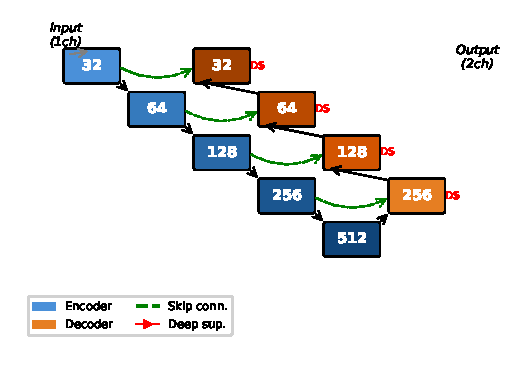
\includegraphics[width=\columnwidth]{figures/unet3d_architecture.pdf}
    \caption{3D U-Net architecture with 5 encoder stages (32--512 channels), residual blocks, strided convolution downsampling, transposed convolution upsampling, skip connections, and deep supervision heads at each decoder level.}
    \label{fig:architecture}
\end{figure}

\subsection{Loss Functions: Topology-Aware Family}

All configurations share the same deep supervision wrapper that applies the base loss at each decoder scale.

\subsubsection{Dice + Cross-Entropy (Baseline)}
The baseline loss combines soft Dice loss with standard cross-entropy. For predicted class probabilities $p_{i,c} = \text{softmax}(z_i)_c$ and one-hot ground truth $g_{i,c}$, the cross-entropy loss is:
\begin{equation}
    \mathcal{L}_{\text{CE}} = -\frac{1}{N}\sum_{i} \sum_{c} g_{i,c} \log p_{i,c}
\end{equation}
where $N$ is the number of voxels and $c$ ranges over classes. The soft Dice loss is computed per foreground class:
\begin{equation}
    \mathcal{L}_{\text{Dice}} = 1 - \frac{2\sum_i p_i g_i + \epsilon}{\sum_i p_i + \sum_i g_i + \epsilon}, \quad \epsilon = 10^{-5}.
\end{equation}
The combined baseline loss is $\mathcal{L}_{\text{base}} = \mathcal{L}_{\text{CE}} + \mathcal{L}_{\text{Dice}}$.

\subsubsection{Dice + CE + Soft-clDice}
Following Shit et al.~\cite{shit2021}, we add a differentiable centerline Dice term. The soft skeleton is extracted iteratively via morphological operations:
\begin{multline}
    \text{skel}(x) = \text{ReLU}\bigl(x - \text{open}(x)\bigr) \\
    + \sum_{k=1}^{K} \text{ReLU}\bigl(\text{erode}^k(x) - \text{open}(\text{erode}^k(x))\bigr)
\end{multline}
with $K=10$. Topology precision and sensitivity are
\begin{align}
    T_{\text{prec}} &= \frac{|\text{skel}(\hat{y}) \cdot y|}{|\text{skel}(\hat{y})|}, \quad
    T_{\text{sens}} = \frac{|\hat{y} \cdot \text{skel}(y)|}{|\text{skel}(y)|}
\end{align}
and $\mathcal{L}_{\text{clDice}} = (1-\alpha)\mathcal{L}_{\text{base}} + \alpha(1 - 2T_{\text{prec}}T_{\text{sens}}/(T_{\text{prec}}+T_{\text{sens}}))$ with $\alpha = 0.5$.

\subsubsection{Dice + CE + Skeleton Recall}
Following Kirchhoff et al.~\cite{kirchhoff2024}, we precompute binary skeletons on CPU using \texttt{skimage.morphology.skeletonize\_3d} and apply a recall-only penalty on centerline voxels:
\begin{equation}
    \mathcal{L}_{\text{skel}} = (1-\alpha)\mathcal{L}_{\text{base}} + \alpha\left(1 - \frac{\sum \hat{y} \cdot \text{skel}(y)}{\sum \text{skel}(y)}\right)
\end{equation}
with $\alpha = 0.5$.

\subsection{Preprocessing and Augmentation}

CTA volumes are clipped to the Hounsfield Unit window $[0, 600]$ and normalized to $[0, 1]$. Multi-class labels are binarized. We use random patch sampling with $128^3$ voxel crops, 4 patches per volume per epoch, and a foreground-centered sampling ratio of 33\%. Augmentation includes random gamma correction ($\gamma \in [0.7, 1.5]$) and random 90-degree axial rotations. Mirror augmentation is disabled to preserve left-right anatomical consistency.

\subsection{Training Procedure}

All models are trained for 300 epochs on 8$\times$NVIDIA A100-SXM4-40GB GPUs using distributed data-parallel (DDP) on an AWS p4d.24xlarge instance. We use AdamW optimizer ($\text{LR}=10^{-3}$, weight decay $10^{-5}$), cosine annealing with 10-epoch linear warmup, batch size 4 per GPU, and mixed-precision training (AMP). Validation runs every 25 epochs with early-stopping patience of 5 cycles. All training configuration is identical across runs to ensure a controlled comparison.

For TopBrain fine-tuning, we load the best from-scratch checkpoint (weights only, fresh optimizer) and train for 150 additional epochs at $10^{-4}$ LR, 5-epoch warmup, same loss. TopBrain's 25 scans (re-annotations of a TopCoW subset) are split 20/5 train/val (seed 42); of the 5 val cases 4 were in TopCoW training (image leakage with sparser labels) and 1 (\texttt{ct\_004}) was in TopCoW val. The TopBrain val therefore primarily measures feature-representation transfer to denser annotations on previously-seen images.

\textbf{Computational cost.} Total wall-clock per configuration (300 from-scratch + 150 TopBrain FT epochs on 8$\times$A100): Dice+CE 65\,min, +clDice 68, +Skeleton 77, +SSIM 75, +MSE-DT \textbf{138}, +Perceptual 73, +Combo 78. All add at most $\sim$15\% over baseline except MSE-DT, whose per-batch CPU \texttt{distance\_transform\_edt} doubles iteration time. Perceptual matches baseline because slice subsampling (stride 16) keeps the VGG batch tiny.

% ============================================================================
\section{Experiments and Results: Topology-Aware Family}

\subsection{Training Dynamics}

Fig.~\ref{fig:learning_curves} shows the training loss and validation Dice progression for the three topology-aware configurations over 300 epochs. The Dice+CE and clDice models exhibit nearly identical loss curves; Skeleton Recall trains at slightly higher loss throughout. Validation Dice plateaus after epoch 200 for all models, with clDice reaching the highest validation Dice (0.864).

\begin{figure}[t]
    \centering
    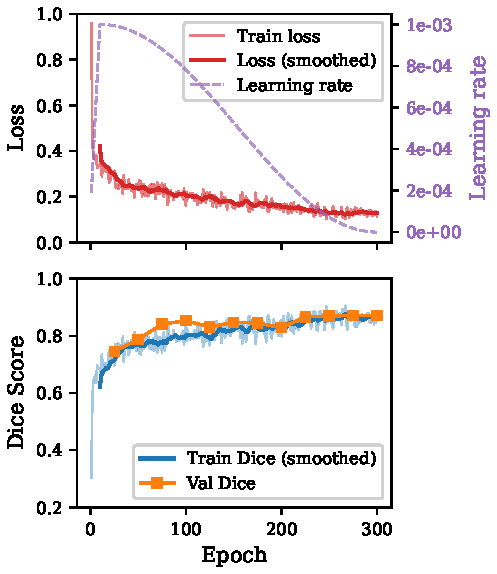
\includegraphics[width=\columnwidth]{figures/learning_curves.pdf}
    \caption{Training dynamics for the three topology-aware loss configurations over 300 epochs on 8$\times$A100 GPUs. \textbf{Top:} Smoothed training loss. \textbf{Bottom:} Smoothed training Dice (lines) and validation Dice (markers, every 25 epochs).}
    \label{fig:learning_curves}
\end{figure}

\subsection{Global Metrics}

\begin{table}[t]
\centering
\caption{Global Evaluation on TopCoW Validation Set --- Topology-Aware Family}
\label{tab:global}
\begin{tabular}{lcccc}
\toprule
\textbf{Model} & \textbf{DSC} & \textbf{clDice} & \textbf{HD95 (mm)} & \textbf{B0 err} \\
\midrule
Dice+CE          & 0.858 & 0.907 & 2.48 & 5.76 \\
Dice+CE+clDice   & \textbf{0.864} & \textbf{0.916} & \textbf{2.40} & \textbf{3.72} \\
Dice+CE+Skeleton & 0.845 & 0.838 & 2.82 & 26.84 \\
\bottomrule
\end{tabular}
\end{table}

The clDice model achieves the highest DSC (0.864), clDice (0.916), and lowest Betti-0 error (3.72). Skeleton Recall trades aggregate overlap for higher communicating-artery recall at the cost of fragmentation (Betti-0 error 26.84).

\subsection{Stratified Per-Vessel Analysis}

\begin{table}[t]
\centering
\caption{Per-Vessel DSC --- Topology-Aware Family. 3rd-A2 has only N=2 cases; differences are not interpretable.}
\label{tab:stratified}
\begin{tabular}{lcccc}
\toprule
\textbf{Vessel} & \textbf{D+CE} & \textbf{+clDice} & \textbf{+Skel.} & \textbf{N} \\
\midrule
BA      & 0.793 & 0.789 & \textbf{0.824} & 25 \\
R-PCA   & 0.802 & \textbf{0.810} & 0.806 & 25 \\
L-PCA   & 0.770 & \textbf{0.809} & 0.793 & 25 \\
R-ICA   & 0.846 & \textbf{0.852} & 0.838 & 25 \\
L-ICA   & \textbf{0.855} & 0.853 & 0.844 & 25 \\
R-MCA   & 0.807 & 0.789 & \textbf{0.806} & 25 \\
L-MCA   & 0.819 & 0.804 & \textbf{0.805} & 25 \\
R-ACA   & 0.725 & \textbf{0.728} & 0.726 & 25 \\
L-ACA   & 0.740 & \textbf{0.741} & \textbf{0.741} & 25 \\
\midrule
Acom    & 0.413 & 0.412 & \textbf{0.415} & 21 \\
R-Pcom  & 0.459 & 0.479 & \textbf{0.511} & 15 \\
L-Pcom  & 0.410 & 0.398 & \textbf{0.479} & 15 \\
3rd-A2  & 0.622 & 0.613 & 0.583 & 2 \\
\bottomrule
\end{tabular}
\end{table}

Aggregating with case-level macro-averaging, the large-vs-communicating DSC gap is 0.363 for both Dice+CE (0.795 vs.\ 0.433) and clDice (0.797 vs.\ 0.435), and 0.332 for Skeleton Recall (0.798 vs.\ 0.466). Skeleton Recall therefore has both the best communicating-artery DSC and the smallest large-vs-communicating gap.

\subsection{TopBrain Fine-Tuning}

\begin{table}[t]
\centering
\caption{TopBrain Fine-Tuned Models: DSC by Vessel Group --- Topology-Aware Family}
\label{tab:topbrain}
\begin{tabular}{lccc}
\toprule
\textbf{Vessel Group} & \textbf{D+CE} & \textbf{+clDice} & \textbf{+Skeleton} \\
\midrule
Large CoW arteries & \textbf{0.832} & 0.829 & 0.821 \\
Communicating      & 0.466 & 0.490 & \textbf{0.513} \\
Distal branches    & 0.687 & 0.712 & \textbf{0.752} \\
Posterior fossa    & 0.565 & 0.533 & \textbf{0.626} \\
Small arteries     & 0.000 & 0.000 & \textbf{0.589} \\
Venous sinuses     & 0.416 & 0.463 & \textbf{0.613} \\
\bottomrule
\end{tabular}
\end{table}

Fine-tuning expands vessel coverage for all three models. The most striking effect is on small arteries (ophthalmic, anterior choroidal): the Skeleton Recall model achieves 0.589 DSC where both alternatives score zero---a qualitative, not merely quantitative, difference. We defer interpretation to §VI.D, which considers two equally compatible explanations (representational prior vs.\ recall-only over-prediction bias).

% ============================================================================
% =====  PAGE 5  ==============================================================
% ============================================================================
\section{Extended Loss Function Investigation}
\label{sec:extended_losses}

We extend the topology-aware ablation with three \emph{reconstruction-aware} losses that operate on the soft probability map rather than its skeleton, each replacing the topology term in the same Dice+CE framework so the only manipulated variable remains the loss.

\subsection{Three Reconstruction-Aware Losses}

Each loss combines the Dice+CE base $\mathcal{L}_{\text{base}}$ with an additional term at $\alpha{=}0.5$. \textbf{Dice+CE+SSIM} adds $(1-\text{SSIM}_{3D}(\hat{p}, g))$ on the softmax foreground probability $\hat{p}$ and one-hot ground truth $g$, computed with a $7^3$ separable Gaussian window ($\sigma{=}1.5$ vox) and standard stabilizers $C_1{=}0.01^2$, $C_2{=}0.03^2$~\cite{wang2004ssim}; this adapts the BASNet recipe~\cite{qin2019basnet} to 3D. \textbf{Dice+CE+MSE-DT} adds MSE on a smooth distance-transform target $t(\mathbf{x}) = \exp(-\text{DT}_{\text{out}}(g)/\sigma)$, $\sigma{=}5$ vox, where $\text{DT}_{\text{out}}$ is the Euclidean distance from each background voxel to the nearest foreground voxel; plain MSE on the raw binary mask collapses on the imbalance, hence the smooth target~\cite{kervadec2021boundary}. The distance transform is computed per patch on CPU under \texttt{torch.no\_grad()}; aggregated over 32 patches per step on 8$\times$A100, this roughly doubles iteration time (see §III.D). \textbf{Dice+CE+Perceptual} adds the L2 distance between frozen ImageNet-pretrained VGG-16~\cite{simonyan2015vgg} features at \texttt{relu2\_2} and \texttt{relu3\_3}, applied per axial slice with stride-16 subsampling; this follows Mosinska et al.~\cite{mosinska2018} and Johnson et al.~\cite{johnson2016perceptual}. We do not modulate by the input CTA (an advanced variant requiring image access inside the loss); the BASNet-style direct probability-map perceptual~\cite{qin2019basnet} keeps the loss interface unchanged. All seven configurations converged stably (Fig.~\ref{fig:learning_curves_extended}); no NaN batches occurred over $\sim$5.7M training samples, and validation DSC clustered tightly from epoch 200 onward.

\begin{figure}[t]
    \centering
    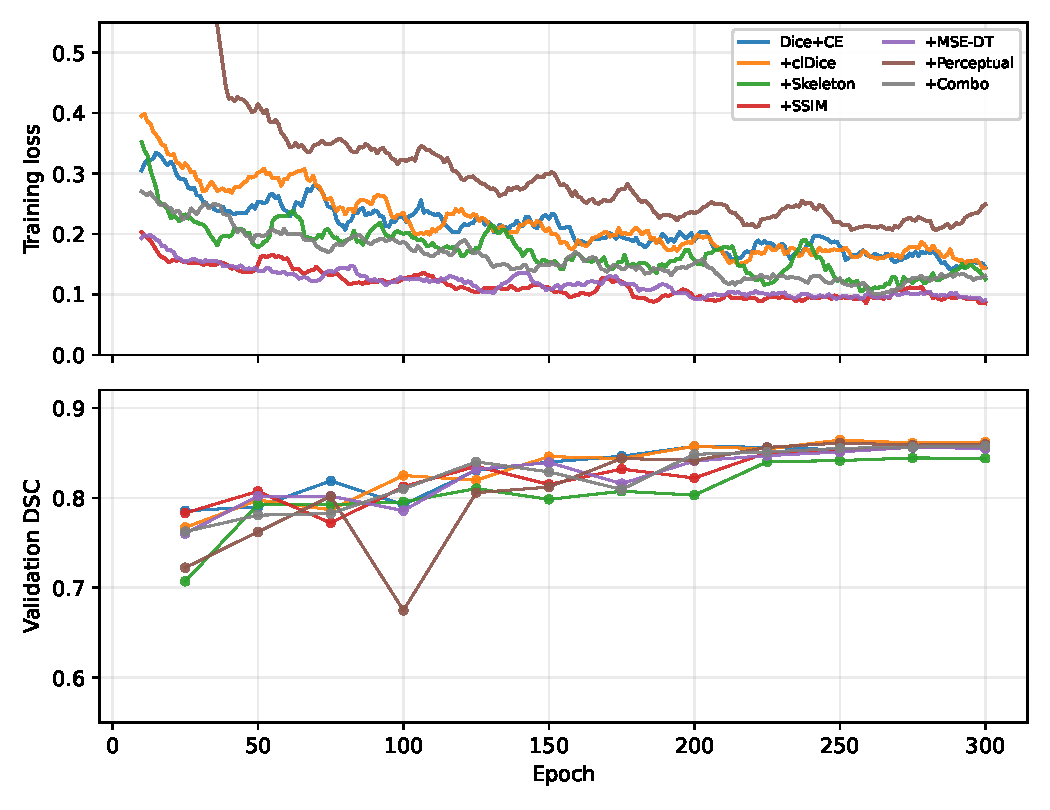
\includegraphics[width=\columnwidth]{figures_v4/learning_curves_extended.pdf}
    \caption{Training loss (top, from epoch 10) and validation DSC (bottom) for all seven configurations on 8$\times$A100. +Perceptual trains at higher absolute loss because the VGG-feature L2 has a different scale.}
    \label{fig:learning_curves_extended}
\end{figure}

% ============================================================================
% =====  PAGE 6  ==============================================================
% ============================================================================
\section{Reconstruction-Aware Evaluation and Combination Loss}
\label{sec:extended_eval}

To characterize each loss along axes orthogonal to overlap and topology, we add three reconstruction-style metrics computed over the same TopCoW validation set, and a final \emph{combination} configuration that merges the best topology-aware and reconstruction-aware terms in a single objective.

\subsection{New Evaluation Metrics}

\noindent\textbf{3D-SSIM} is computed on the binary prediction vs.\ binary GT using a Gaussian window ($\sigma{=}1.5$ vox); higher is better. Because most voxels are background, absolute SSIM is high ($\sim$0.99); we report it for relative ranking.

\noindent\textbf{PSNR} (in dB) is $-10\log_{10}\text{MSE}(\hat{y}_b, g_b)$ on the binary prediction; higher is better, capped at 100.

\noindent\textbf{Fr\'echet Feature Distance (F-FID)} is computed at the set level: VGG-16 \texttt{relu3\_3} features over axial slices of all validation predictions and ground truths (stride 16) are pooled and the Fr\'{e}chet distance between the two empirical Gaussians reported. We label this \emph{F-FID, not FID}, because $N{=}25$ is far below the sample size at which the original Inception-FID metric was demonstrated to converge; it is a feature-space proxy useful for ranking, not for absolute fidelity.

\subsection{Combination Loss: Dice + CE + clDice + SSIM}

The combination configuration $\mathcal{L}_{\text{combo}} = 0.5\,\mathcal{L}_{\text{base}} + 0.25\,\mathcal{L}_{\text{clDice}}^* + 0.25\,\mathcal{L}_{\text{SSIM}}^*$ tests whether topology-aware and reconstruction-aware supervision compound. It is trained from scratch on TopCoW with the identical pipeline as all other configurations and fine-tuned on TopBrain.

\subsection{Extended Results Table}

\begin{table*}[t]
\centering
\caption{Extended evaluation on TopCoW validation set (N=25). Higher is better except HD95, B0 err, and F-FID. Bold = best in column; ties jointly bolded. Per-volume standard deviations are 6--12\% of the mean for DSC/clDice and 5--40\% for B0 err.}
\label{tab:extended}
\begin{tabular}{lccccccc}
\toprule
\textbf{Model} & \textbf{DSC}$\uparrow$ & \textbf{clDice}$\uparrow$ & \textbf{HD95 (mm)}$\downarrow$ & \textbf{B0 err}$\downarrow$ & \textbf{3D-SSIM}$\uparrow$ & \textbf{PSNR (dB)}$\uparrow$ & \textbf{F-FID}$\downarrow$ \\
\midrule
Dice+CE                       & 0.858 & 0.907 & 2.48 & 5.76  & 0.9986 & 39.09 & \textbf{0.0017} \\
Dice+CE+clDice                & \textbf{0.864} & \textbf{0.916} & \textbf{2.40} & \textbf{3.72}  & \textbf{0.9987} & \textbf{39.24} & \textbf{0.0017} \\
Dice+CE+Skeleton              & 0.845 & 0.838 & 2.82 & 26.84 & 0.9982 & 38.59 & 0.0054 \\
Dice+CE+SSIM                  & 0.856 & 0.903 & 2.54 & 6.72  & 0.9986 & 39.03 & 0.0018 \\
Dice+CE+MSE-DT                & 0.857 & 0.893 & 2.89 & 7.48  & 0.9985 & 38.96 & 0.0022 \\
Dice+CE+Perceptual            & 0.861 & 0.902 & 2.51 & 6.88  & 0.9986 & 39.13 & \textbf{0.0017} \\
Dice+CE+clDice+SSIM (combo)   & 0.858 & 0.910 & 2.57 & 4.12  & 0.9986 & 39.04 & 0.0018 \\
\bottomrule
\end{tabular}
\end{table*}

Paired two-sided Wilcoxon signed-rank tests across the 25 validation cases (\texttt{scipy.stats.wilcoxon}, default zero-handling), with Holm-Bonferroni correction at family-wise $\alpha{=}0.05$ across six pairwise contrasts per metric, sharpen the picture. \emph{All results below characterize the $\alpha{=}0.5$ convex form only}; weight sweeps and curriculum schedules were not tested. On the centerline-Dice metric, clDice is significantly better than five of the six other configurations under Holm correction (vs.\ Skeleton, MSE-DT, Perceptual, SSIM, baseline; raw $p$ from $4{\times}10^{-5}$ to $0.019$); the sixth comparison, vs.\ Combo, fails to reach significance ($p{=}0.30$). On DSC, only clDice vs.\ Skeleton survives correction ($p{=}0.0004$, capturing the fragmentation cost we report in §IV.B and §VI.D); clDice is \emph{not} significantly different from MSE-DT ($p{=}0.05$, above Holm threshold $0.010$), SSIM ($p{=}0.06$), baseline ($p{=}0.14$), Combo ($p{=}0.22$), or Perceptual ($p{=}0.37$). The topology-aware loss wins on the centerline metric; the DSC story is not a clDice-vs-baseline gain but rather a clDice-vs-Skeleton overlap loss for the latter.

The three reconstruction-aware losses produce SSIM, PSNR, and F-FID values within the per-case noise floor of the baseline (per-volume $\sigma{\approx}0.0006$ on SSIM, $\sim$2\,dB on PSNR; mean differences are an order of magnitude smaller). At $\alpha{=}0.5$, the reconstruction term does not measurably move the corresponding metric---attributable to background dominance (binary CTA masks are $>$95\% background, pinning SSIM and PSNR near saturation). The BASNet (BCE+SSIM+IoU) template~\cite{qin2019basnet}, developed for natural-image salient-object detection with diverse backgrounds, was tested here in the closest analogue (Dice+CE+SSIM); it contributes negligibly in 3D medical CTA. Our Perceptual variant also fails to replicate the topological-correctness improvement reported by Mosinska et al.~\cite{mosinska2018}; we attribute the gap to setting differences (their 2D natural-image delineation vs.\ our 3D medical CTA, and direct optimization on tubular masks vs.\ our slice-wise frozen-VGG probability-map variant).

The combination $(0.5, 0.25, 0.25)$ is numerically worse than clDice alone on every metric, but the difference fails to reach significance on either DSC ($p{=}0.22$) or the centerline metric ($p{=}0.30$). The conservative reading: combo \emph{does not significantly exceed} clDice; we cannot distinguish the two. On F-FID, clDice ties with baseline and Perceptual at 0.0017---a three-way numerical tie consistent with noise-floor clustering, not a clDice-specific win. One plausible mechanism for the combo's failure to compound is that the SSIM term, without useful gradient signal of its own, consumes 25\% of the weight that would otherwise reinforce clDice; we leave this as a hypothesis since we did not run the targeted weight-sweep ablation. A constructive combination at lower SSIM weight or with a curriculum schedule is plausible but untested.

\subsection{TopBrain Transfer: Skeleton Recall Retains the Small-Vessel Advantage}

\begin{table}[t]
\centering
\caption{TopBrain Fine-Tuned Models: DSC by Vessel Group --- All Seven Configurations (best per row in bold; on Large CoW SSIM is best at 0.834, only 0.002 above the Dice+CE baseline at 0.832).}
\label{tab:topbrain_extended}
\setlength{\tabcolsep}{3.2pt}
\footnotesize
\begin{tabular}{lccccccc}
\toprule
\textbf{Group} & \textbf{D+CE} & \textbf{+cl} & \textbf{+Sk} & \textbf{+S} & \textbf{+M} & \textbf{+P} & \textbf{+C} \\
\midrule
Large CoW       & 0.832 & 0.829 & 0.821 & \textbf{0.834} & 0.823 & 0.825 & 0.831 \\
Communicating   & 0.466 & 0.490 & \textbf{0.513} & 0.461 & 0.465 & 0.469 & 0.489 \\
Distal branches & 0.687 & 0.712 & \textbf{0.752} & 0.674 & 0.683 & 0.706 & 0.714 \\
Posterior fossa & 0.565 & 0.533 & \textbf{0.626} & 0.541 & 0.526 & 0.551 & 0.558 \\
Small arteries  & 0.000 & 0.000 & \textbf{0.589} & 0.000 & 0.000 & 0.011 & 0.000 \\
Venous sinuses  & 0.416 & 0.463 & \textbf{0.613} & 0.425 & 0.456 & 0.481 & 0.450 \\
\bottomrule
\multicolumn{8}{l}{\scriptsize Columns: D+CE = Dice+CE; +cl = +clDice; +Sk = +Skeleton;}\\
\multicolumn{8}{l}{\scriptsize +S = +SSIM; +M = +MSE-DT; +P = +Perceptual; +C = +Combo.}
\end{tabular}
\end{table}

Table~\ref{tab:topbrain_extended} extends Table~\ref{tab:topbrain} to all seven configurations on the TopBrain validation set ($N{=}5$). Skeleton+TB wins five of six vessel groups and is uniquely the only model that segments small arteries at all (0.589 DSC); among the four reconstruction-aware variants, only Perceptual produces any non-zero output (0.011), with SSIM, MSE-DT, and Combo at zero. The cost of Skeleton's coverage is fragmentation: $\sim$1752 connected components on average versus 130--280 for every other configuration. We do not invoke TopBrain F-FID values here given $N{=}5$; the component ratio is the primary evidence. Two interpretations are equally compatible with this transfer advantage: a representational prior toward thin tubular geometry, or the recall-only objective biasing the network toward over-prediction that survives fine-tuning. Distinguishing them requires a follow-up we did not run (e.g., Skeleton Recall with an added FP penalty).

\begin{figure}[t]
    \centering
    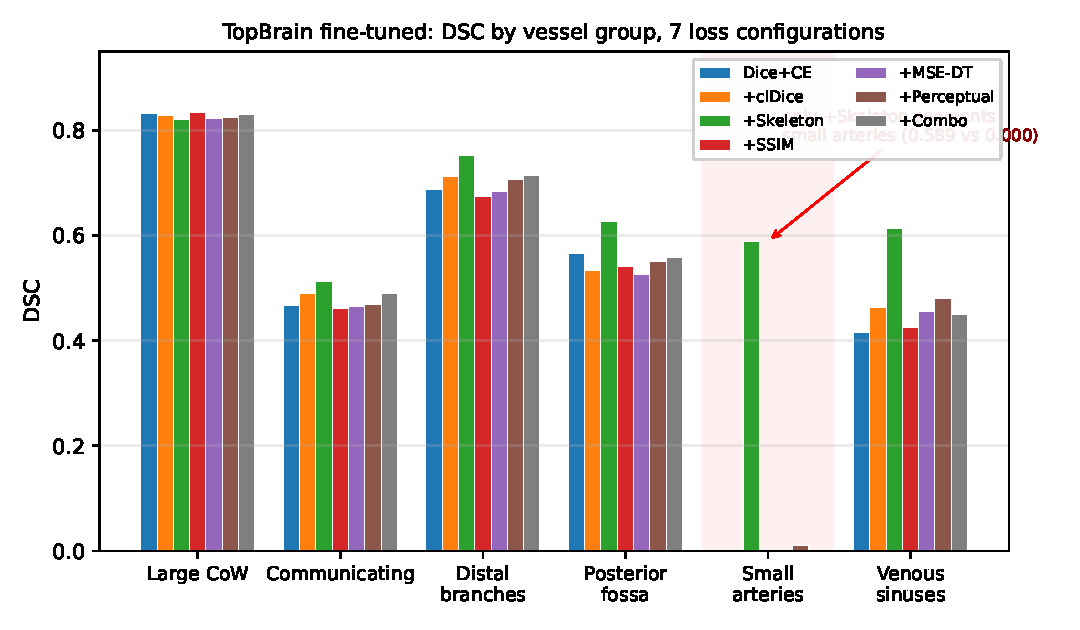
\includegraphics[width=\columnwidth]{figures_v4/topbrain_extended_groups.pdf}
    \caption{TopBrain fine-tuned DSC by vessel group across all seven configurations. Skeleton Recall (green) wins five of six groups; on small arteries, it is the only model that segments these structures at all (0.589 vs.\ $\leq$0.011 for every other model).}
    \label{fig:topbrain_extended}
\end{figure}

\enlargethispage{2\baselineskip}

% ============================================================================
\section{Conclusion}

At $\alpha{=}0.5$, Holm-corrected Wilcoxon tests show clDice as the only loss producing statistically distinguishable centerline-metric improvement (vs.\ five of six others); on DSC only clDice $>$ Skeleton survives.

Mapped to our three hypotheses: (i) is partially supported and splits within the topology-aware family---Skeleton Recall numerically helps Pcom at the cost of global fragmentation, while on Acom all three topology-aware configurations cluster within 0.003 (no meaningful effect). (ii) cannot be adjudicated by our binary-mask reconstruction metrics, which saturate against $>$95\% background; the topology half (``does not recover topology'') is consistent with our data, but soft probability-map fidelity remains untested. (iii) is falsified at equal weights: the clDice+SSIM combination produces no measurable improvement over clDice alone.

Skeleton Recall is uniquely able to segment the smallest cerebral arteries after TopBrain transfer ($N{=}5$; see §III.D for image-leakage caveat). Future work: $\alpha$-sweeps, an FP-penalized Skeleton Recall variant, and multi-class artery/vein segmentation.

% ============================================================================
\bibliographystyle{IEEEtran}

% Compact bibliography to keep total at 6 pages (IEEE conference). The
% font size and itemsep changes have to be applied INSIDE the
% thebibliography environment because IEEEtran resets to \normalsize
% on \begin{thebibliography}.
\begin{thebibliography}{16}
\scriptsize
\setlength{\itemsep}{-0.3ex}
\setlength{\parsep}{0pt}
\setlength{\parskip}{0pt}

\bibitem{isensee2021}
F.~Isensee, P.~F.~Jaeger, S.~A.~A.~Kohl, J.~Petersen, and K.~H.~Maier-Hein,
``nnU-Net: A self-configuring method for deep learning-based biomedical image segmentation,''
\textit{Nature Methods}, vol.~18, pp.~203--211, 2021.

\bibitem{yang2023}
K.~Yang \textit{et al.},
``Benchmarking the CoW with the TopCoW challenge: Topology-aware anatomical segmentation of the Circle of Willis for CTA and MRA,''
\textit{arXiv:2312.17670}, 2023.

\bibitem{shit2021}
S.~Shit \textit{et al.},
``clDice---A novel topology-preserving loss function for tubular structure segmentation,''
in \textit{Proc. IEEE/CVF CVPR}, pp.~16560--16569, 2021.

\bibitem{isensee2024}
F.~Isensee \textit{et al.},
``nnU-Net revisited: A call for rigorous validation in 3D medical image segmentation,''
in \textit{Proc. MICCAI}, 2024.

\bibitem{kirchhoff2024}
Y.~Kirchhoff \textit{et al.},
``Skeleton Recall Loss for connectivity conserving and resource efficient segmentation of thin tubular structures,''
in \textit{Proc. ECCV}, 2024.

\bibitem{shi2024cbd}
P.~Shi \textit{et al.},
``Centerline Boundary Dice Loss for vascular segmentation,''
in \textit{Proc. MICCAI}, 2024.

\bibitem{berger2024}
A.~Berger \textit{et al.},
``Topologically faithful multi-class segmentation in medical images,''
in \textit{Proc. MICCAI}, 2024.

\bibitem{wang2004ssim}
Z.~Wang, A.~C.~Bovik, H.~R.~Sheikh, and E.~P.~Simoncelli,
``Image quality assessment: From error visibility to structural similarity,''
\textit{IEEE Trans.\ Image Process.}, vol.~13, no.~4, pp.~600--612, 2004.

\bibitem{qin2019basnet}
X.~Qin, Z.~Zhang, C.~Huang, C.~Gao, M.~Dehghan, and M.~Jagersand,
``BASNet: Boundary-Aware Salient Object Detection,''
in \textit{Proc. IEEE/CVF CVPR}, pp.~7479--7489, 2019.

\bibitem{mosinska2018}
A.~Mosinska, P.~Marquez-Neila, M.~Koziński, and P.~Fua,
``Beyond the pixel-wise loss for topology-aware delineation,''
in \textit{Proc. IEEE/CVF CVPR}, pp.~3136--3145, 2018.

\bibitem{kervadec2021boundary}
H.~Kervadec, J.~Bouchtiba, C.~Desrosiers, E.~Granger, J.~Dolz, and I.~Ben~Ayed,
``Boundary loss for highly unbalanced segmentation,''
\textit{Medical Image Analysis}, vol.~67, p.~101851, 2021.

\bibitem{johnson2016perceptual}
J.~Johnson, A.~Alahi, and L.~Fei-Fei,
``Perceptual losses for real-time style transfer and super-resolution,''
in \textit{Proc. ECCV}, pp.~694--711, 2016.

\bibitem{simonyan2015vgg}
K.~Simonyan and A.~Zisserman,
``Very deep convolutional networks for large-scale image recognition,''
in \textit{Proc. ICLR}, 2015.

\end{thebibliography}

\end{document}
